\section{Design}
The system will be a frontend for a user to interact with the SpaceTraders API through a console prompt and graphical interface. And is described by the structure chart below:


\shadowbox{
    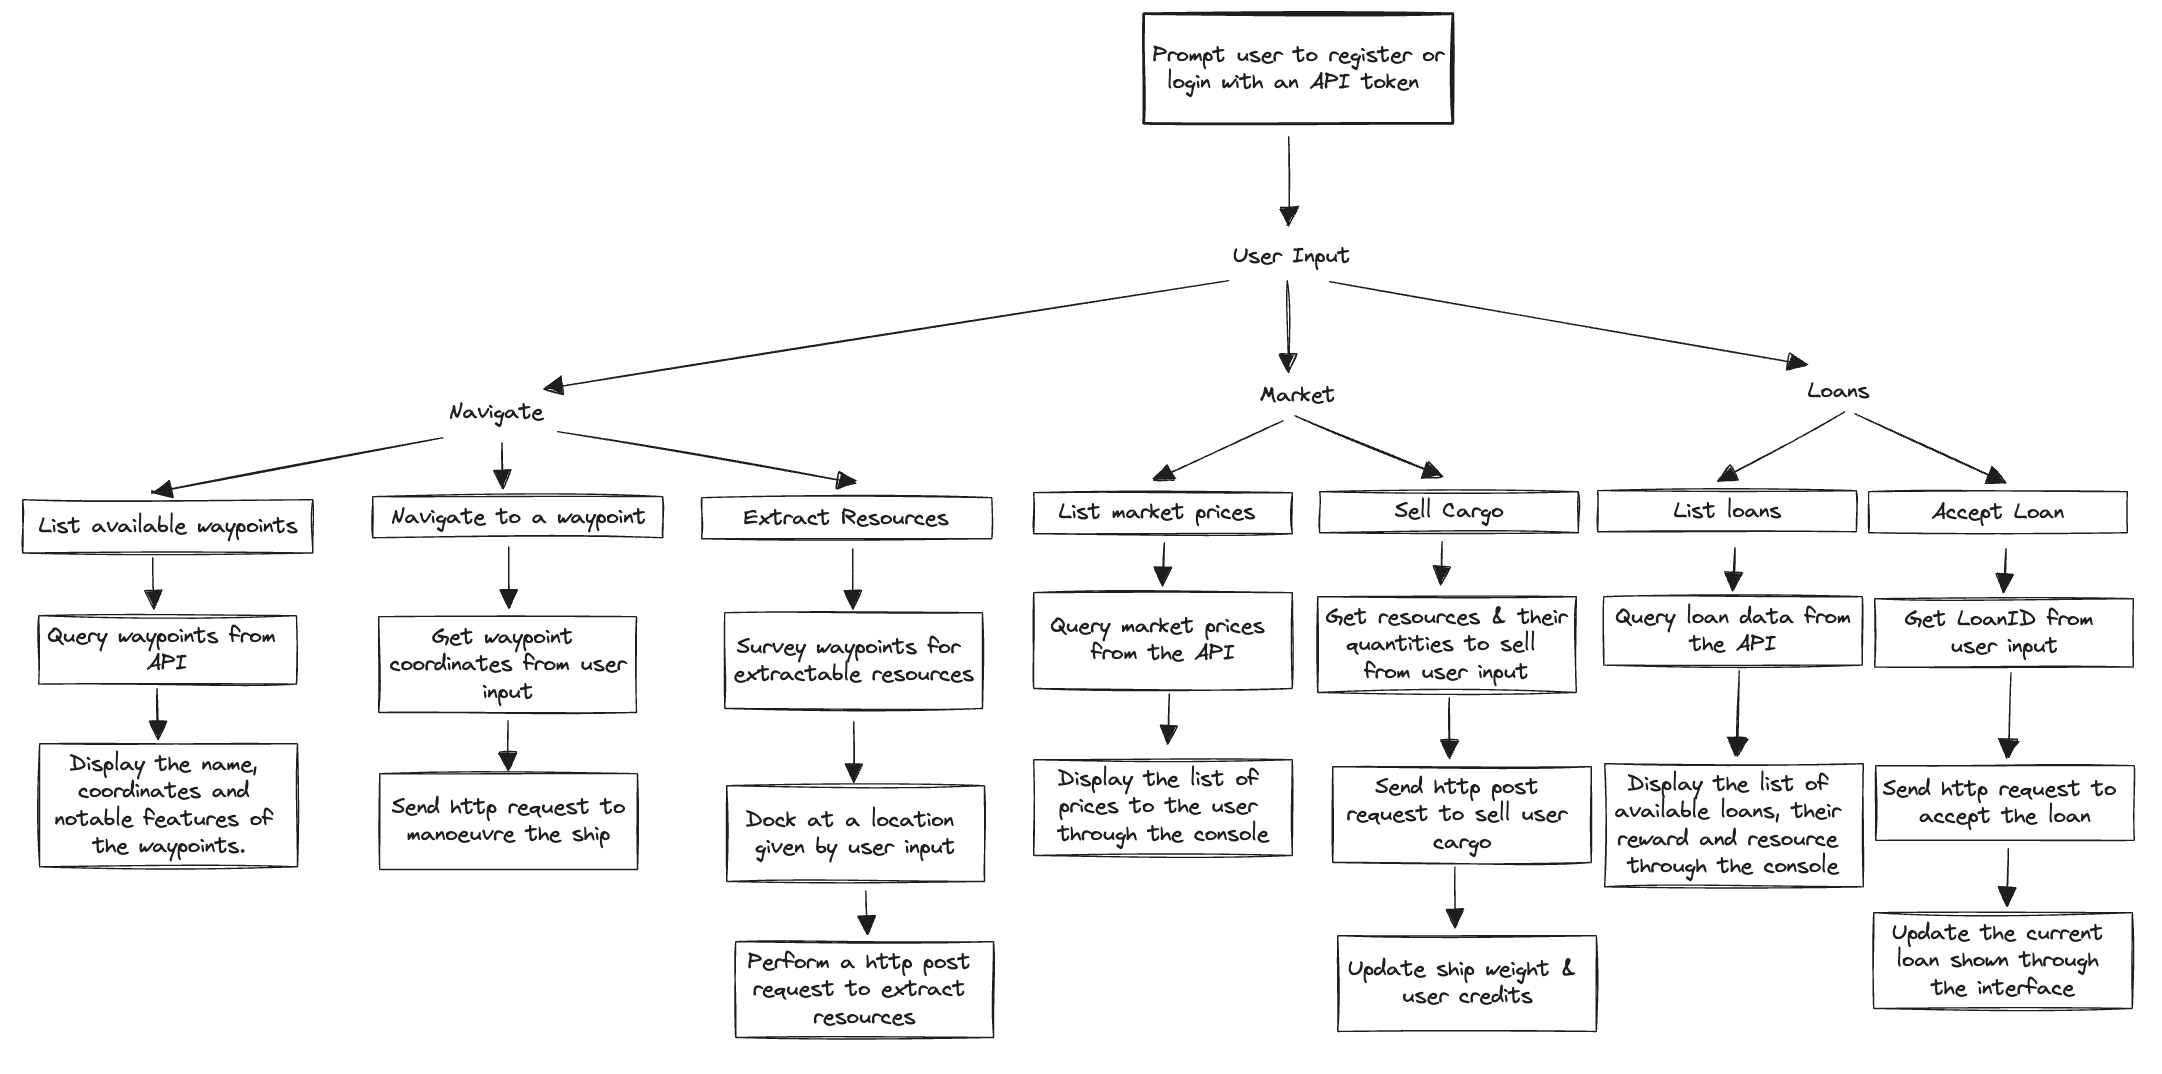
\includegraphics[angle=90, origin=c, width=12cm]{system-diagram.png}
}

\subsection{Data Design}
I will parse the JSON responses from http requests into a series of structs which can be passed as parameters to maintain state. A \texttt{GameState} class will hold references to the other classes required for API calls, or communicating information to the user and will be defined as below. The waypoints vector will be used for displaying a graphical star map on the right of the screen, and the Agent reference, for storing the symbolic name and token key for future API requests.
\begin{lstlisting}
struct GameState {
    agent: &Agent,
    waypoints: Vec<Waypoint>,
}
\end{lstlisting}

The Agent class will store all account information that may be displayed through the interface or required for API calls, including: the agent's symbolic name, API token, current loan, and credits. It also contains a vector of Ships composing the fleet, thus mitigating the need for querying the API every time information is requested – and the structs only have to be rebuilt when performing modifying requests – thus reducing latency by minimising requests.

\begin{lstlisting}
struct Agent {
    token: &str, 
    symbol: &str,
    credits: u32,
    curr_loan: &Loan,
    fleet: Vec<Ship>,
} 
\end{lstlisting}

The Agent class contains references to both the \texttt{Ship}, and \texttt{Loan} classes defined by the specification below. Both will be created to parse the json response of a request into an organised structure, and stored to later be queried when users request information on their fleet or loans.

\begin{lstlisting}
enum FlightMode {
    CRUISE,
    BURN,
    DRIFT,
    STEALTH,
}

struct Ship {
    flight_mode: FlightMode,
    curr_waypoint: &Waypoint,
    fuel: i32,
    curr_weight: u32,
    max_weight: u32,
}

enum Resource {
    IRON_ORE,
    COPPER_ORE,
}

struct Loan { 
    reward: i32,
    resource: Resource,
    expiration_date: DateTime,
}
\end{lstlisting}

A similar interface definition of the \texttt{Waypoint} struct can be created. Instances of these will be stored in a vector attribute of the \texttt{GameState} struct, and used to visually display a map of the star system, as well as to be referenced by ships to indicate their current position.

\begin{lstlisting}
enum Trait {
    SHIPYARD,
    MARKET,
    ASTEROID
}

struct Waypoint {
    symbol: &str,
    coordinate: [i64; 2],
    trails: Vec<Trait>,
}
\end{lstlisting}